\uuid{7R8x}
\exo7id{7142}
\titre{exo7 7142}
\auteur{megy}
\organisation{exo7}
\datecreate{2017-04-05}
\isIndication{true}
\isCorrection{true}
\chapitre{Géométrie affine euclidienne}
\sousChapitre{Géométrie affine euclidienne du plan}
\module{Géométrie}
\niveau{L2}
\difficulte{}

\contenu{
\texte{
Soient deux cercles se coupant en deux points distincts $A$ et $B$, et $\mathcal D$ une tangente commune, touchant les cercles en $C$ et $D$. Montrer que $(AB)$ coupe $[CD]$ en son milieu.
\begin{center}
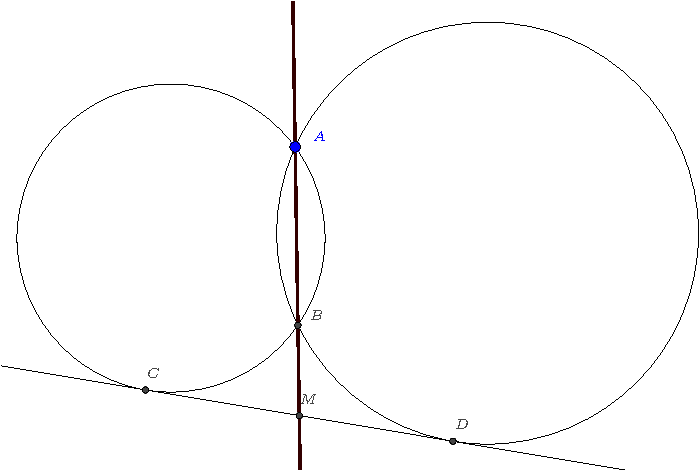
\includegraphics{../images/7R8x-1}
\end{center}
}
\indication{Considérer les puissances par rapport aux deux cercles.}
\reponse{
Rappelons la figure:

\begin{center}
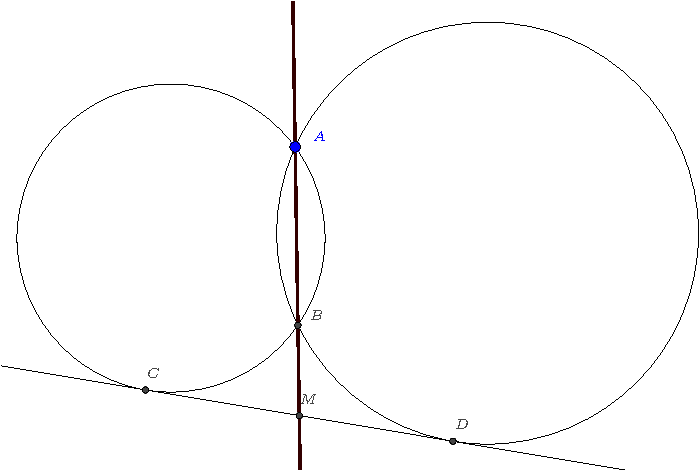
\includegraphics{../images/7R8x-1}
\end{center}

Soit $M$ un point de $(AB)$. Sa puissance par rapport aux deux cercles est la même et vaut $\overrightarrow{MA}\cdot \overrightarrow{MB}$.
 
Par ailleurs, si $M$ est de plus sur la tangente commune $(CD)$, alors sa puissance par rapport au premier cercle est $MC^2$, et celle par rapport au deuxième cercle est $MD^2$. On en déduit que $MC=MD$, donc $M$ est le milieu de $[CD]$.
}
}
